\documentclass[portrait,plainboxedsections]{sciposter}

\usepackage{amsmath}
\usepackage{amssymb}
\usepackage{booktabs}
\usepackage{graphicx}
\usepackage{microtype}

\newcommand{\earlywarning}{early-warning}
\newcommand{\GW}{{\sc gw}}
\newcommand{\EM}{{\sc em}}
\newcommand{\GRB}{{\sc grb}}
\newcommand{\CBC}{{\sc cbc}}
\newcommand{\LIGO}{{\sc ligo}}
\newcommand{\LCGT}{{\sc lcgt}}
\newcommand{\GEO}{{\sc geo600}}
\newcommand{\ISCO}{{\sc isco}}
\newcommand{\SNR}{{\sc snr}}
\newcommand{\realtime}{real-time}
\newcommand{\Msun}{\ensuremath{M_{\odot}}}
\newcommand{\order}[1]{\ensuremath{\mathcal{O}[#1]}}
\newcommand{\tmpsamps}{\ensuremath{N}}
\newcommand{\numtmps}{\ensuremath{M}}
\newcommand{\numslices}{\ensuremath{S}}
% macros for number of svd basis functions
\newcommand{\SVD}{{\sc svd}}
\newcommand{\svdtmps}[1]{\ensuremath{L^#1}}
\newcommand{\numsvdtmps}{\svdtmps{s}}
% macros for sample points in slices
\newcommand{\slicesamps}[1]{\ensuremath{N^#1}}
\newcommand{\slicessamps}{\slicesamps{s}}
\newcommand{\fftblock}{\ensuremath{D}}
\newcommand{\resampsamps}{\ensuremath{N^\shortdownarrow,\, N^\shortuparrow}}
\newcommand{\fir}{{\sc fir}}
\newcommand{\fft}{{\sc fft}}
\newcommand{\fmax}{\ensuremath{f^0}}
\newcommand{\flops}{flop/s}
\newcommand{\gstlal}{{\tt gstlal}}
\newcommand{\gstreamer}{{\tt GStreamer}}
\newcommand{\numcpus}{{600}}
\newcommand{\lloid}{{\sc lloid}}
\newcommand{\TD}{{\sc td}}
\newcommand{\FD}{{\sc fd}}

% Macros for collapsing sizes of things
% From TUGboat, Volume 22 (2001), No. 4
% http://www.tug.org/TUGboat/tb22-4/tb72perlS.pdf
\def\clap#1{\hbox to 0pt{\hss#1\hss}}
\def\mathllap{\mathpalette\mathllapinternal}
\def\mathrlap{\mathpalette\mathrlapinternal}
\def\mathclap{\mathpalette\mathclapinternal}
\def\mathllapinternal#1#2{\llap{$\mathsurround=0pt#1{#2}$}} 
\def\mathrlapinternal#1#2{\rlap{$\mathsurround=0pt#1{#2}$}} 
\def\mathclapinternal#1#2{\clap{$\mathsurround=0pt#1{#2}$}}

% Colors for signal flow diagram and equation
\def\diagramcolorfir{red}
\def\diagramcolorreconstruct{blue}
\def\diagramcoloraccum{red!50!yellow}

% customize colors
\definecolor{BoxCol}{RGB}{0,35,102} % RoyalBlue
\definecolor{SectionCol}{RGB}{255,255,255} % White


\title{Toward early-warning detection of compact binary coalescence}

\author{\textsc{Nickolas V. Fotopoulos}, Leo Singer}

\institute{LIGO Laboratory, California Institute of Technology}

\email{foton@caltech.edu}

\begin{document}
\conference{Amaldi 9, Cardiff, Wales, UK; This document bears the DCC number LIGO-G1100683-v1.}

\maketitle

\begin{minipage}[t]{0.25\textwidth}

\section*{Motivation}

\PARstart{B}acon ipsum dolor sit amet reprehenderit minim tongue, pork nostrud
ham hock ea est salami shoulder commodo bresaola tenderloin pork belly id.
Fugiat sausage cillum in nostrud. Jowl consequat ground round, non incididunt
rump excepteur tongue voluptate pork loin ut brisket velit veniam. Dolore non
magna, pork belly voluptate eiusmod ut anim. Quis qui cow biltong, in ea salami
reprehenderit pork belly. Sirloin do shankle minim elit. Sunt fugiat t-bone
corned beef ut, excepteur aliqua eu meatloaf.
%
\begin{figure}[h]
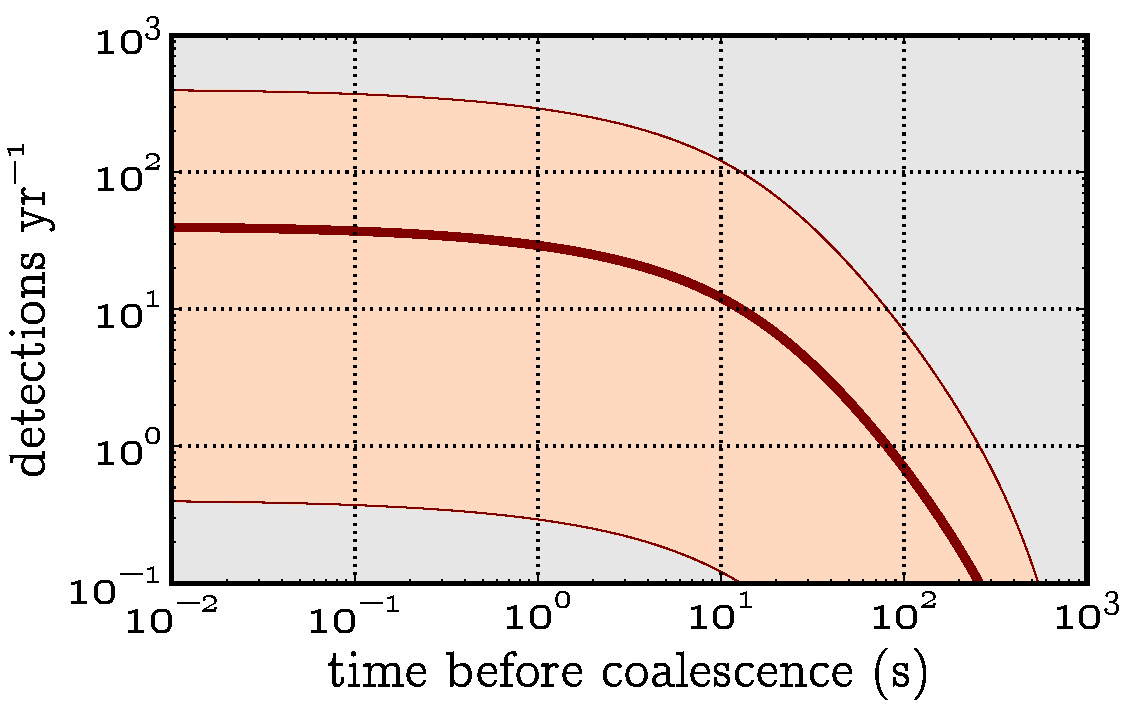
\includegraphics{figures/snr_in_time}
\caption{\label{fig:earlywarning}Expected number of \textsc{ns}--\textsc{ns}
sources that could be detectable by Advanced \LIGO\ a given number of seconds
before coalescence.  The heavy solid line is the most realistic yearly rate
estimate.  The shaded region represents the 5 to 95\% confidence interval
arising from uncertainty in predicted event rates \cite{Abadie:2010p10836}.}
\end{figure}
%
\begin{figure}[h]
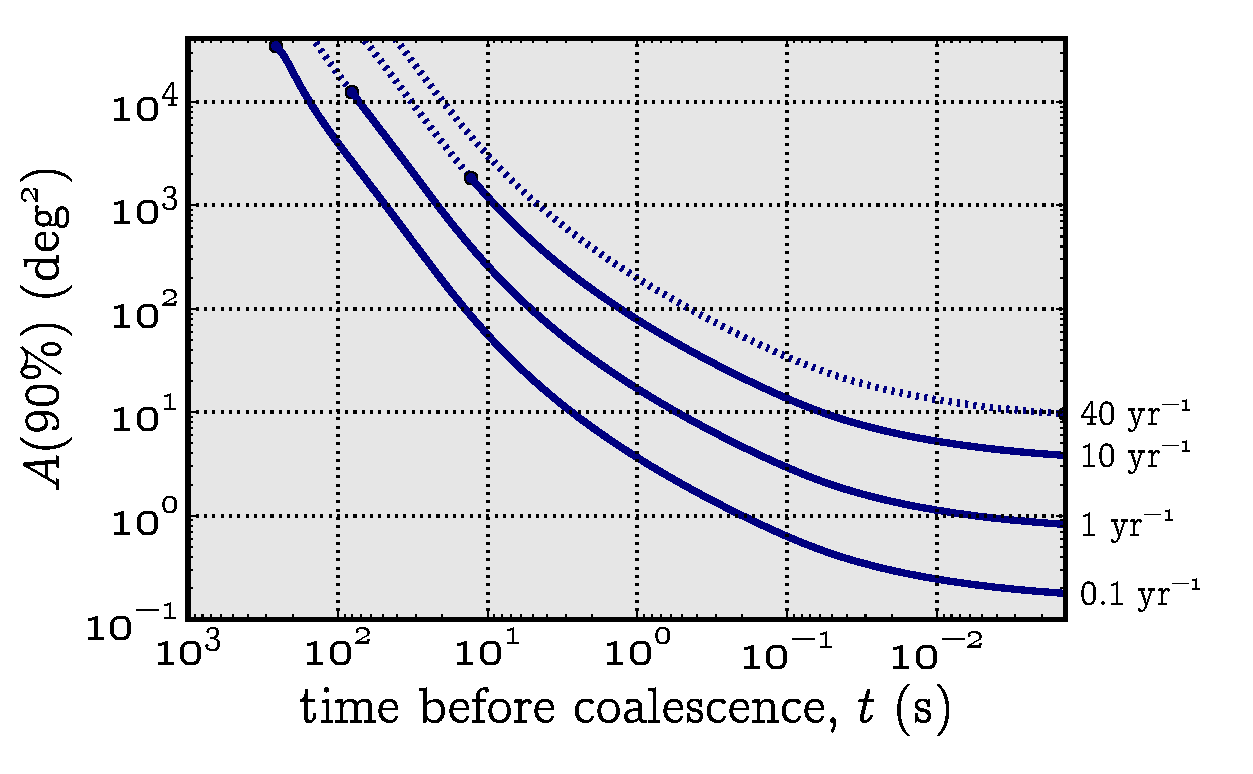
\includegraphics{figures/loc_in_time}
\caption{\label{fig:sky-localization-accuracy}Area of the 90\% confidence
region as a function of time before coalescence for sources with anticipated
detectability rates of 40, 10, 1, and 0.1~yr$^{-1}$. The heavy dot indicates
the time at which the accumulated \SNR\ exceeds a threshold of~8.}
\end{figure}

Et shoulder tongue commodo corned beef. Flank ground round mollit est, in
salami do swine meatloaf aliqua non pancetta ham ea. Ut salami id venison rump
esse. Incididunt ribeye occaecat, short loin beef sint bacon cupidatat
hamburger shank. Ribeye eiusmod strip steak, drumstick pariatur enim spare ribs
t-bone meatloaf aliquip bacon occaecat sunt pork chop. Drumstick commodo jerky
pork loin incididunt, ground round beef ribs. Fatback elit ground round
drumstick ribeye, ham mollit adipisicing labore bresaola.

\begin{figure}
%\includegraphics{olapredfcn}
%\put(-450,350){\huge Placeholder}
\caption{Latency time-line}
\label{f:latency_timeline}
\end{figure}

Incididunt tempor commodo adipisicing nisi nulla, short ribs ham non dolor
nostrud spare ribs cow. Enim rump anim eu deserunt officia, veniam shankle
meatloaf et. Chicken id voluptate cupidatat bacon chuck. Incididunt salami elit
pork loin pork chop. Tail chicken qui boudin. Tail dolor do, laboris in id
meatloaf consectetur salami beef anim. Ad pork chop irure, sausage excepteur
deserunt labore.

Eu ground round laboris pancetta adipisicing. Quis flank aliquip bacon jowl et.
Minim pig occaecat magna, tenderloin venison beef. Sint aute chicken corned
beef. Ball tip ea bresaola proident. In qui cillum in excepteur dolor dolore.
Non pork loin shankle magna.

\end{minipage}%
\hspace{0.05\textwidth}%
\begin{minipage}[t]{0.4\textwidth}

\begin{figure}[h!]
	\begin{center}
		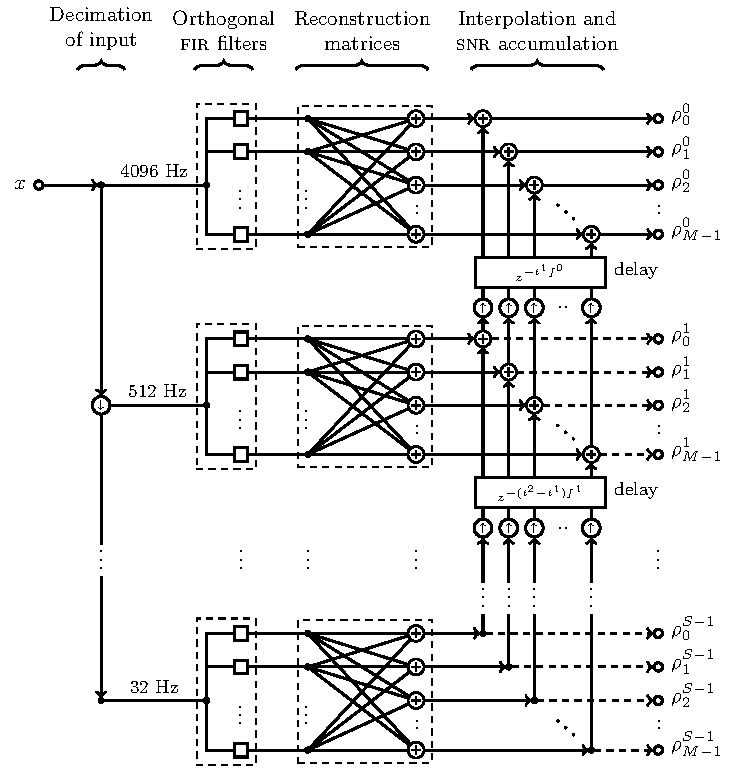
\includegraphics[width=\textwidth]{figures/lloid-diagram}
		\caption{\label{fig:pipeline} Schematic of \lloid{} pipeline illustrating
signal flow.  Circles with arrows represent interpolation
\protect
\includegraphics[scale=3]{figures/upsample-symbol} or decimation
\protect
\includegraphics[scale=3]{figures/downsample-symbol}.  Circles with plus
signs represent summing junctions
\protect
\includegraphics[scale=3]{figures/adder-symbol}.  Squares
\protect
\includegraphics[scale=3]{figures/fir-symbol} stand for \fir{} filters.  Sample
rate decreases from the top of the diagram to the bottom.  In this diagram each
time slice contains three \fir\ filters that are linearly combined to produce
four output channels.  In a typical pipeline the number of \fir\ filters is
much less than the number of output channels.}
	\end{center}
\end{figure}

\begin{multline}
	\rho_i^s [k] =%
		% Interpolation SNR
		\overbrace{
			\left(H^\uparrow \rho_i^{s+1}\right)[k]
		}^\textrm{\clap{{\sc snr} from previous time slices}} \\
		% Plus ...
		+
		% Reconstruction
		\underbrace{
			\sum_{\mathclap{l=0}}^{\mathclap{L^s-1}} v_{il}^s \sigma_l^s
		}_\textrm{\clap{reconstruction}}
		% Orthogonal FIR filter
		\overbrace{
			\sum_{\mathclap{n=0}}^{\mathclap{N^s-1}} u_l^s[n] x^s[k-n]
		}^\textrm{\clap{orthogonal {\sc fir} filters}} .
\end{multline}

\section*{Results}

\PARstart{A}liquip elit excepteur ut in. Sirloin in pork venison flank. Sausage reprehenderit ball tip dolor venison excepteur bresaola culpa, fatback chuck proident strip steak meatball short loin tongue. Labore pork beef ribs short loin nisi ea. Pastrami laborum nostrud incididunt ut officia. Pancetta elit rump, swine shoulder brisket sunt short ribs eu cow short loin irure anim culpa. Laborum deserunt mollit pork belly rump ground round.

\end{minipage}%
\hspace{0.05\textwidth}%
\begin{minipage}[t]{0.25\textwidth}

\section*{Implementation}

\begin{figure}[h]
	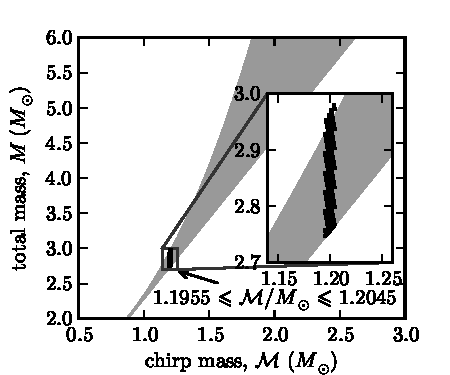
\includegraphics{figures/tmpltbank}
	\caption{\label{fig:tmpltbank}Source parameters selected for sub-bank used in this
case study, consisting of component masses $m_1$, $m_2$, between 1 and 3~$M_\odot$, and
chirp masses $\mathcal{M}$ between 1.1955 and 1.2045~$M_\odot$.}
\end{figure}

\begin{figure}
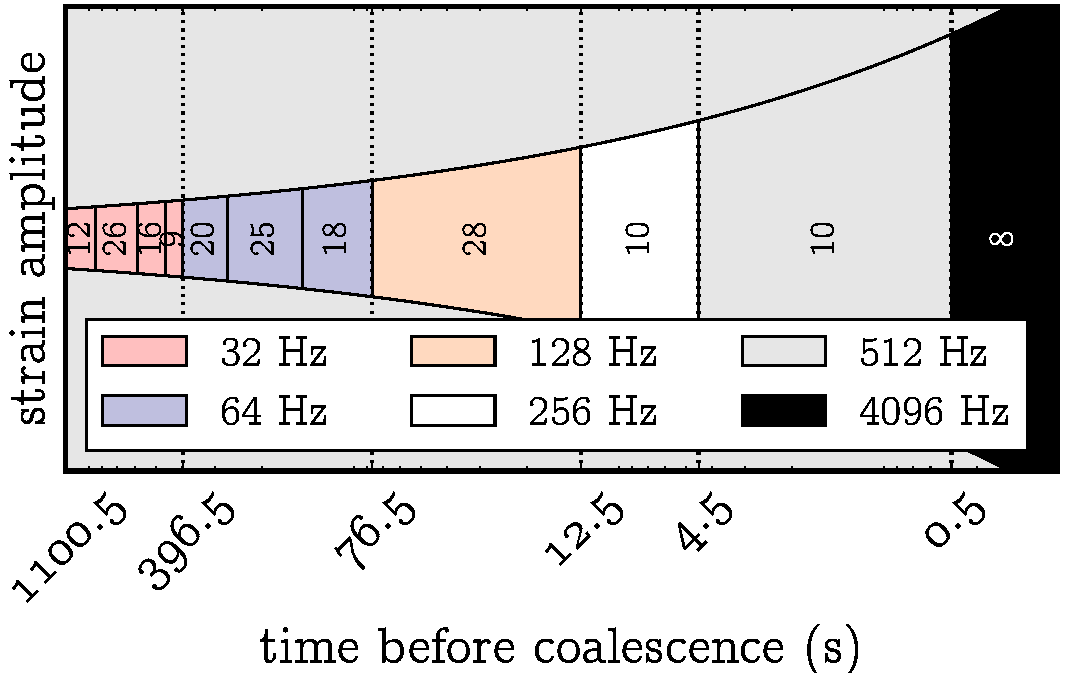
\includegraphics{figures/envelope}
\caption{envelope}
\end{figure}

\begin{table}
\begin{tabular}{rr@{,\,}lcc}
\toprule
\\ [-2ex]
$f^s$ & $[t^s$&$t^{s+1})$ & & \\% [1ex]
\\[-2.5ex]
(Hz) & \multicolumn{2}{c}{(s)} & $N^s$ & $L^s$ \\ \midrule
4096 & [0&0.5) & 2048 & 8 \\
512 & [0.5&4.5) & 2048 & 10 \\
256 & [4.5&12.5) & 2048 & 10 \\
128 & [12.5&76.5) & 8192 & 28 \\
64 & [76.5&140.5) & 4096 & 18 \\
64 & [140.5&268.5) & 8192 & 25 \\
64 & [268.5&396.5) & 8192 & 20 \\
32 & [396.5&460.5) & 2048 & 9 \\
32 & [460.5&588.5) & 4096 & 16 \\
32 & [588.5&844.5) & 8192 & 26 \\
32 & [844.5&1100.5) & 8192 & 12 \\
\bottomrule
\end{tabular}
\caption{\label{tab:time_slices} Filter design sub-bank of 657 templates.  From left to right, this table shows the sample rate, time interval, number of samples, and number of orthogonal templates for each time slice.  We vary \SVD{} tolerance from $\left(1-10^{-1}\right)$ to $\left(1-10^{-6}\right)$.}
\end{table}


\begin{figure}
\centering
%\includegraphics{olapredfcn}
%\put(-450,350){\huge Placeholder}
%\includegraphics{likelihoods}
\caption{GStreamer pipeline.}
\label{f:gstreamer_pipeline}
\end{figure}

\end{minipage}

\section*{Acknowledgements}

\LIGO\ was constructed by the California Institute of Technology and
Massachusetts Institute of Technology with funding from the National Science
Foundation and operates under cooperative agreement
\textsc{phy}-\oldstylenums{0107417}. This research
is supported by the National Science Foundation through a Graduate Research
Fellowship to LS.

%%% References

\bibliographystyle{plain}
\bibliography{biblio}

\end{document}
